\documentclass{sig-alternate}
\usepackage{graphicx}
\usepackage{url}
\usepackage{amssymb}
\usepackage[usenames,dvipsnames]{color}

\newcommand{\gd}[1]{\textcolor{ForestGreen}{GD: #1}}
\newcommand{\amt}[1]{Amazon MTurk}

\begin{document}
%
% --\item Author Metadata here ---
\conferenceinfo{WWW}{'15}
%\CopyrightYear{2007} % Allows default copyright year (20XX) to be over-ridden \item IF NEED BE.
%\crdata{0-12345-67-8/90/01}  % Allows default copyright data (0-89791-88-6/97/05) to be over-ridden \item IF NEED BE.
% --\item End of Author Metadata ---

% \title{The Evolution of Micro-task Crowdsourcing Markets}
\title{The Dynamics of Micro-Task Crowdsourcing}
\subtitle{The Case of Amazon MTurk}
% The Evolution of Micro-Task Crowdsourcing Markets —- The Case of Amazon Mechanical Turk
% The Dynamics of Micro-Task Crowdsourcing -- The Case of Amazon MTurk
% Anatomy of a Micro-Task Crowdsourcing Platform
% Unravelling Micro-Task Crowdsourcing Dynamics/Processes
% The Market for HITs: Throughput Uncertainty and the Market Mechanism


\numberofauthors{1}
\author{
\alignauthor
Djellel E. Difallah$^*$, Michele Catasta$^\dagger$, Gianluca Demartini$^\ddagger$, \\  Panagiotis G. Ipeirotis$^\diamond$, Philippe Cudr\'e-Mauroux$^*$\\
       \affaddr{$^*$ eXascale Infolab, University of Fribourg, Switzerland}\\
       \affaddr{$^\dagger$ EFPL, Switzerland}\\
       \affaddr{$^\ddagger$ University of Sheffield, UK}\\
	   \affaddr{$^\diamond$ New York University, USA}
       % \email{trovato@corporation.com}
}

\maketitle
\begin{abstract}
Micro-task crowdsourcing is rapidly gaining popularity among research communities and businesses as a means to leverage Human Computation in their daily operations. Unlike any other ``technology'', a crowdsourcing platform is subject to human factors that affect its performance, both in terms of speed and quality. Indeed, such factors shape the \emph{dynamics} of the crowdsourcing market. For example, a known behavior of such markets is that increasing the reward of a task would lead to faster results. However, it is still unclear how different dimensions interact each other: reward, task type, market competition, requester reputation, etc.

In this paper we adopt a data-driven approach to perform a long-term analysis of a popular micro-task crowdsourcing platform to understand behavior evolution of its main actors: workers, requesters, tasks, and platform. We leverage the main findings of our five year log analysis to generate features used in a predictive model for the expected performance of a batch of tasks published on the crowdsourcing platform at a specific point in time by a certain requester.
\end{abstract}

% A category with the (minimum) three required fields
\category{H.4}{Information Systems Applications}{Miscellaneous}
%A category including the fourth, optional field follows...
% \category{D.2.8}{Software Engineering}{Metrics}[complexity measures, performance measures]

\terms{Design, Experimentation, Human Factors}

\keywords{Crowdsourcing, human computation, log analysis}

%!TEX root = ../dynamics.tex
\section{Introduction}\label{sec:intro}
The micro-task crowdsourcing market has seen a rapid growth in the last five years. This is correlated with the fact that more data is available to enterprises and that data is an asset within business processes. While data is available, its quality is not always high and manual processing is often necessary. To this end, outsourcing  data processing tasks  like image tagging, audio transcription, translation, etc. to a large crowd of individuals has become popular.

%micro-task Crowdsourcing platform
To perform such Human Intelligence Tasks (HITs) crowdsourcing platforms have been developed. Such platforms serve as place where the crowd (i.e., people willing to perform small tasks in exchange of a small monetary reward, also know as \emph{workers}) and work providers (i.e., also known as \emph{requesters}) meet. \gd{describe crowdsourcing process of publishing tasks, completing task, getting results, rewarding}

%
In this paper we analyze the evolution of a very popular micro-task crowdsourcing platform over the last five years and propose techniques to support requesters in posting HITs to the market in an effective way. Using features derived from a large-scale analysis of platform logs, we propose methods to predict the throughput of the crowdsourcing platform for a batch of HITs published by a certain requester at a certain point in time. This prediction is based on different features including current platform load, requester reputation, popular task types, etc.

\gd{summarize main findings}


In summary, the main contributions of this paper are:
\begin{itemize}

	\item An analysis of the evolution of a popular micro-task crowdsourcing market looking at dimensions like topics, task types, reward, worker location.

	\item A large-scale classification of 2.5M HITs published on Amazon MTurk.

	\item An effective model to predict the completion speed of a batch published on Amazon MTurk at a certain point by a certain requester.

	\item An online service with evolution statistics and services for requesters to better design their HIT metadata (e.g., keywords, reward, etc.)

\end{itemize}


The rest of the paper is structured as follows.
In Section \ref{sec:relwork} we overview recent work on micro-task crowdsourcing specifically focusing on works improving efficiency of crowdsourcing systems.
%!TEX root = ../dynamics.tex
\section{Related Work}\label{sec:relwork}

\subsection{Micro-task Crowdsourcing}

A very popular platform is Amazon MTurk\footnote{\url{http://mturk.com}} which provides access to a crowd of workers distributed worldwide but mainly composed of people based in USA and India \cite{mturk}.

Workers share experiences about HITs and requesters within web forums and ad-hoc websites \cite{turkopticon}. Such requester `reviews' serve as a way to measure requester reputation which is assumed to be a reason for obtaining answers efficiently from the crowd \cite{}. In this work we experimentally show the effect of platform and requester properties on crowd efficiency.  \gd{rephrase last sentence?}


\subsection{Human Computation}
Micro-task crowdsourcing is used to improve the quality of purely machine-based systems in order to combine both the scalability of machines over large amounts of data as well as the quality of human intelligence to process and understand data.
Many examples of such hybrid approaches exist.
Crowd-powered databases \cite{crowddb} leverage crowdsourcing to deal with incomplete data, complex data integration problems, graph search, and joins \cite{crowder,graphsearch,crowdjoins}.
Semantic Web systems leverage the crowd for schema matching \cite{crowdmap}, entity linking \cite{zencrowd}, and ontology engineering \cite{bioonto}.
Information Retrieval systems use crowdsourcing for evaluation purposes \cite{mizzaroalonso}.

When building systems that build on top of crowdsourcing platforms, two main challenges have to be dealt with: effectiveness and efficiency  of the crowd.

\subsection{Crowdsourcing Effectiveness}

A very important dimension for crowdsourcing effectiveness is \emph{answer aggregation}, that is, after assigning the same HIT to multiple workers in the crowd, effectively aggregate their answers in a final results to be output back from the crowdsourcing platform to the system leveraging human computation. Multiple approaches have been proposed for this aspect of crowdsourcing quality (e.g.,
\cite{Venanzi:2014:CBA:2566486.2567989,square,zencrowd,Hosseini:2012:ALM:2260641.2260661}).
% 
A recent approach which results in effective aggregation is \cite{Venanzi:2014:CBA:2566486.2567989} where authors detect communities of workers with similar answering patterns to re-weight their answers even when little evidence of individual worker quality is available (i.e., just few HITs have been completed).


More than aggregation, identifying the best worker in the crowd is another mean to obtain quality answers from the crowd \cite{pickacrowd,bozzon}.

More recently, \cite{Jung14-hcomp} aims at predicting work quality looking at worker activities over time.

\subsection{Crowdsourcing Efficiency}

In \cite{Kittur:2013:FCW:2441776.2441923} authors provide their view on how the crowdsourcing market should adapt specifically focusing on how to  support full-time crowd workers. On the other hand, in this work we perform a data-driven analysis of the evolution of micro-task crowdsourcing over the past five years using the findings of such analysis as features to support requesters while publishing HITs on these platforms in an effective way.

\cite{finishthem,scaleup}

To improve human computation efficiency, it is key to support worker in being more efficient while working on HITs. For example, workers spend way too much time in searching for HITs to work on \cite{Kucherbaev:2014:TET:2598153.2602249}.






% final remark
Our work is complementary to existing work as we present a data-driven study of the evolution of micro-task crowdsourcing over five years as a support evidence of the ongoing efforts to improve crowdsourcing quality and efficiency that we have described.



%!TEX root = ../dynamics.tex
\section{The Evolution of Amazon MTurk\\ From 2009 to 2014}
\label{sec:stats}

We start by describing our datasets and extract some key information that will be used in the rest of the paper.

\subsection{Crowdsourcing Platform Dataset}
\label{sec:tracker}
Over the past five years, we have periodically collected data about HITs being published on \amt{}.
Real-time data that we collected from the platform is available at \url{http://mturk-tracker.com/}. In this work, we consider hourly aggregated data that includes the available HIT batches and their metadata (tittle, description, rewards, required qualifications, etc.), in addition to their progress over time, that is, the temporal variation of the set of HITs available. In fact, one of the main metrics that we leverage (see Section \ref{sec:throughput}) is the throughput of a batch, i.e., how many HITs  get completed between two successive observations; Our initial intuition in this context, backed by Figure \ref{fig:motiv}, is that the throughput of a batch is heavily tied to its number of HITs that are currently available to workers.\\
In total, our dataset covers more than 2.5M different batches with over 130M HITs.
We note that the tracker reports data periodically only and does not reflect fine-grained information (e.g., variations at each second). We believe however that it captures enough information to perform meaningful, long-term trend analyses and to understand the dynamics and interactions within the crowdsourcing platform.\\

\begin{figure}[tb]
	\centering
		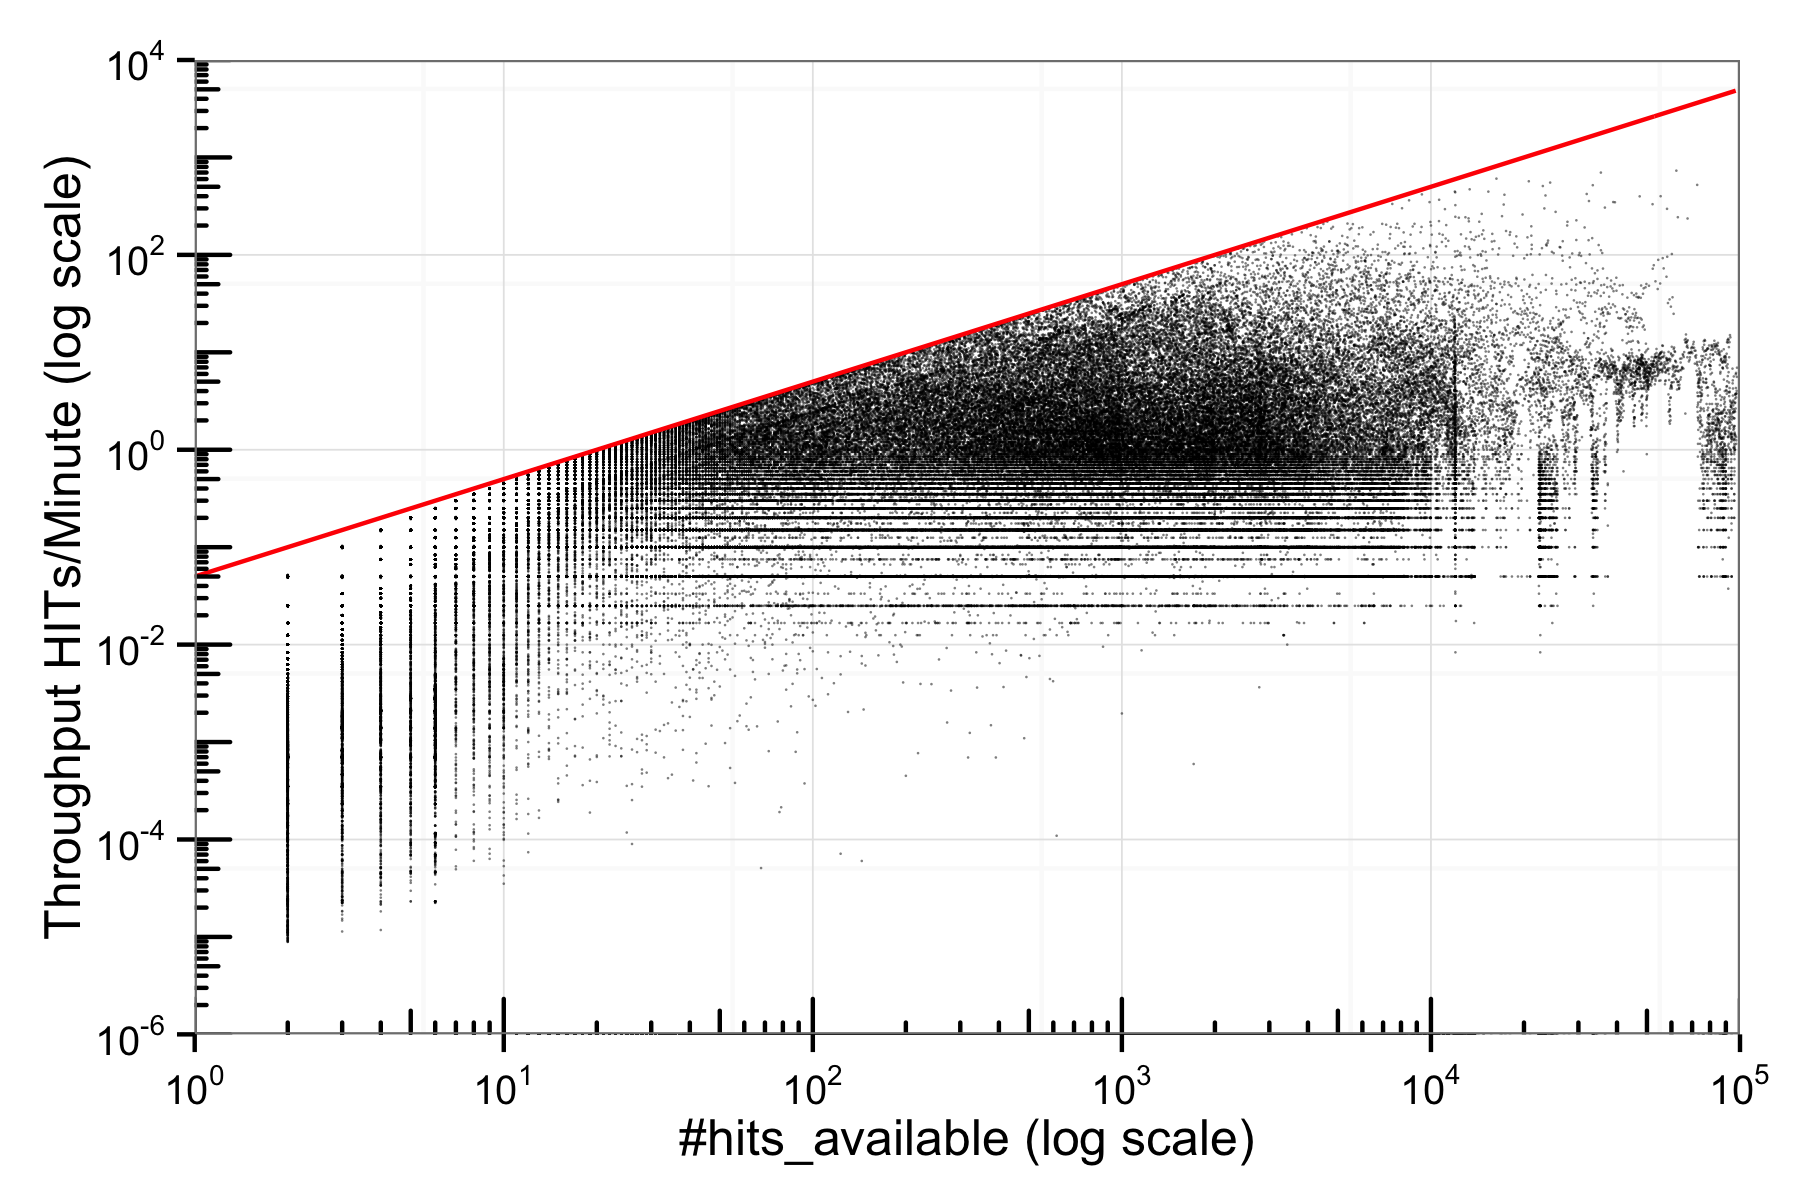
\includegraphics[width=0.48\textwidth]{figures/motiv_mturk}
	\caption{Batch throughput versus the number of HITs available in the batch. The red line corresponds to the maximum throughput we could have observed due to the tracker periodicity constraints.\protect\footnotemark}
	\label{fig:motiv}
\end{figure}
\begin{figure}[tb]
	\centering
		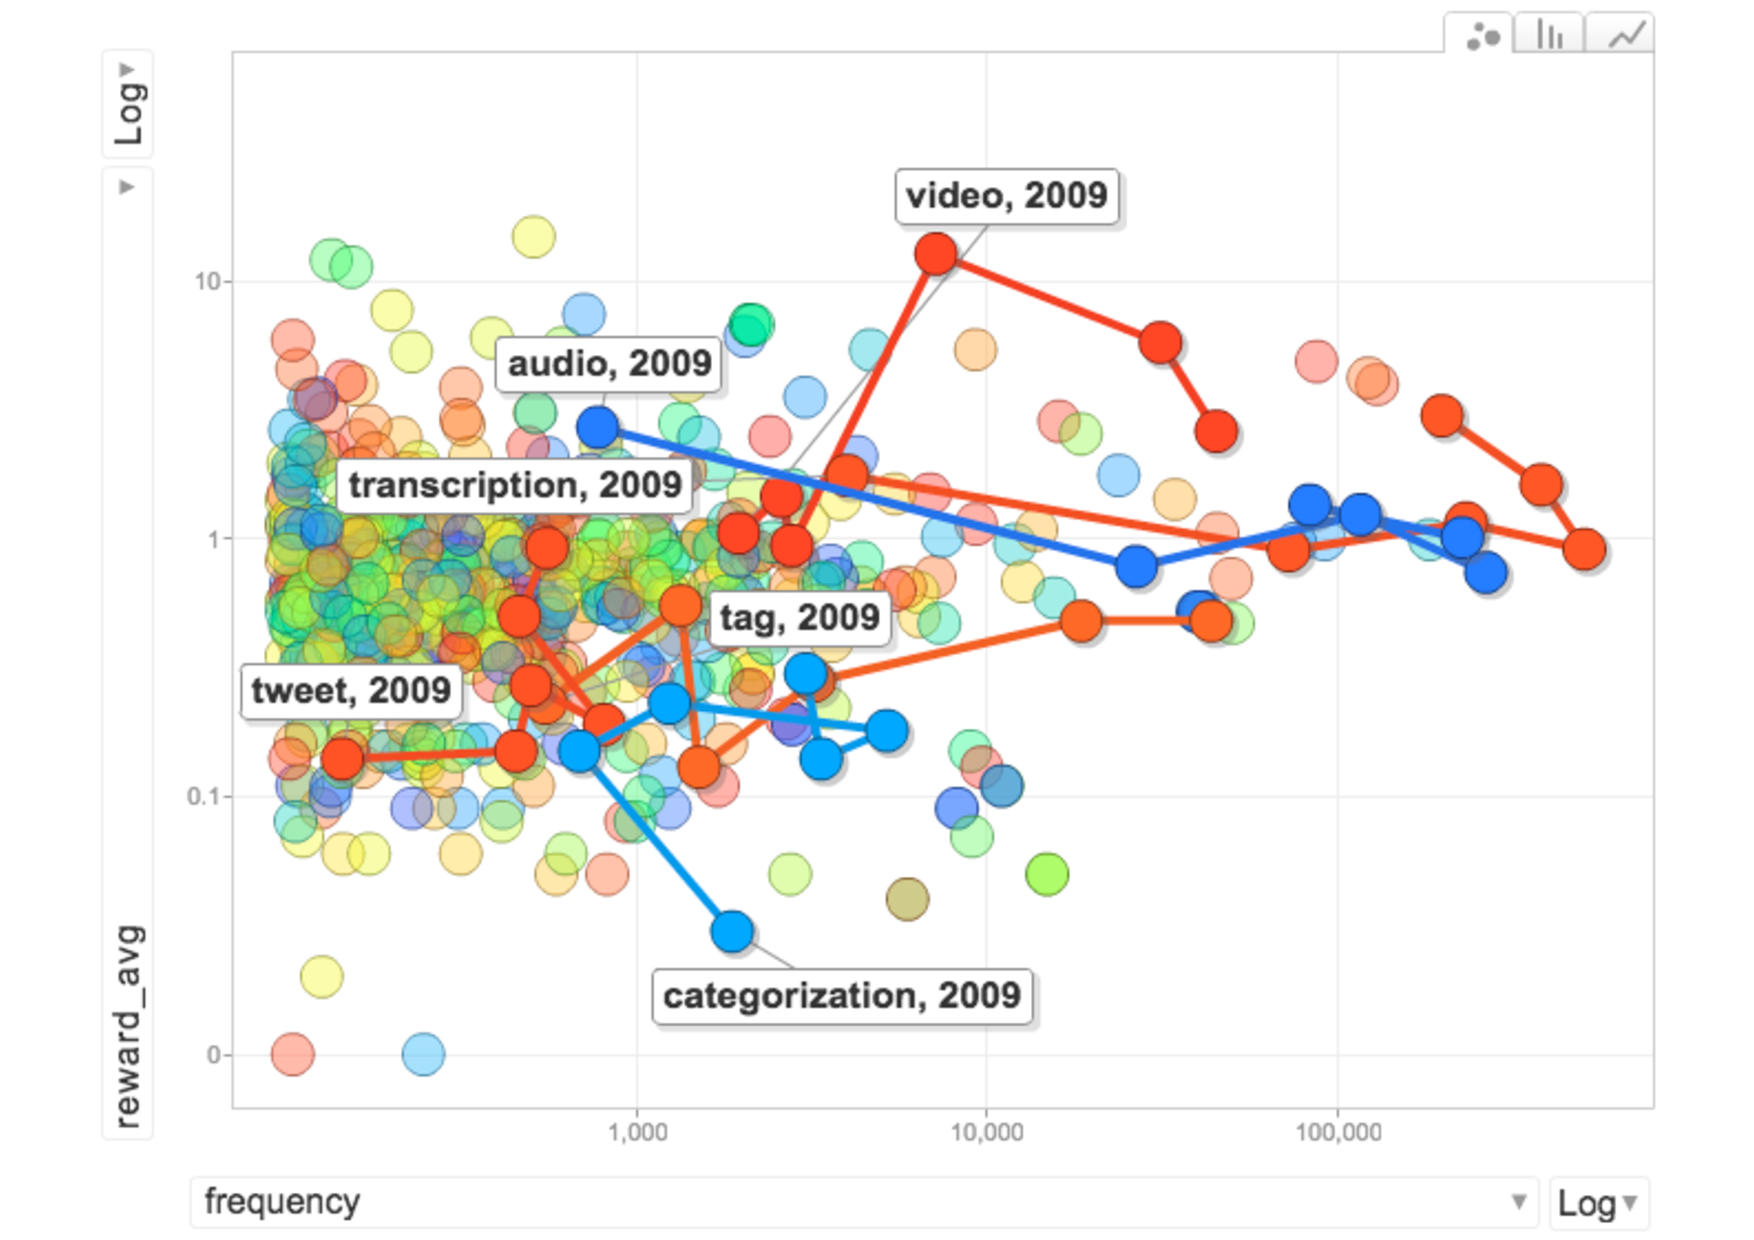
\includegraphics[width=0.5\textwidth]{figures/tagEvolution}
	\caption{The use of keywords to annotate HITs. $frequency$ corresponds to how many times a keyword was used, and $reward\_avg$ corresponds to the average monetary reward of batches that listed the keyword.}
	\label{fig:tagEvolution}
\end{figure}

\subsection{A Data-driven Analysis of Platform Evolution}
First, we identify the trends obtained from aggregated information over time, keywords or countries associated with the published HITs.  Each of the following analyses is also available as an interactive visualization over the historical data on \url{http://xi-lab.github.io/mturk-mrkt/}.
\paragraph{Topics  Over Time}
First we want to understand how different topics have been addressed by means of micro-task crowdsourcing over time.
In order to do this analysis, we look at the keywords associated with published HITs. We observe the evolution of keyword popularity and associated reward on \amt{}. 
%plot explanation
Figure \ref{fig:tagEvolution} shows this behavior. Each point in the plot represents a keyword associated to the HITs with its frequency (i.e., number of HITs with this keyword) on the x-axis, and the average reward in a given year on the y-axis. The path connecting data points indicates the time evolution, starting in 2009, with one point representing the keyword usage over one year.

% observations
We observe that the `audio' and `transcription' keywords (i.e., blue and red paths from left to right) have substantially increased in frequency over time. They have become the most popular keywords in the last two years and are paid more than \$1 on average.
HITs with the `video' tag have also increased in number with a reward that has reached a peak in 2012 and decreased after that.
HITs tagged as `categorization' have been paid consistently in the range of \$0.10-\$0.30 on average, except in 2009 where they were rewarded less than \$0.10 each.
HITs tagged as `tweet' have not increased in number but have been paid more over the years, reaching \$0.9 on average in 2014: This can be explained by more complex tasks being offered to workers, such as sentiment classification or writing tweets.

\begin{figure*}[tb]
	\centering
		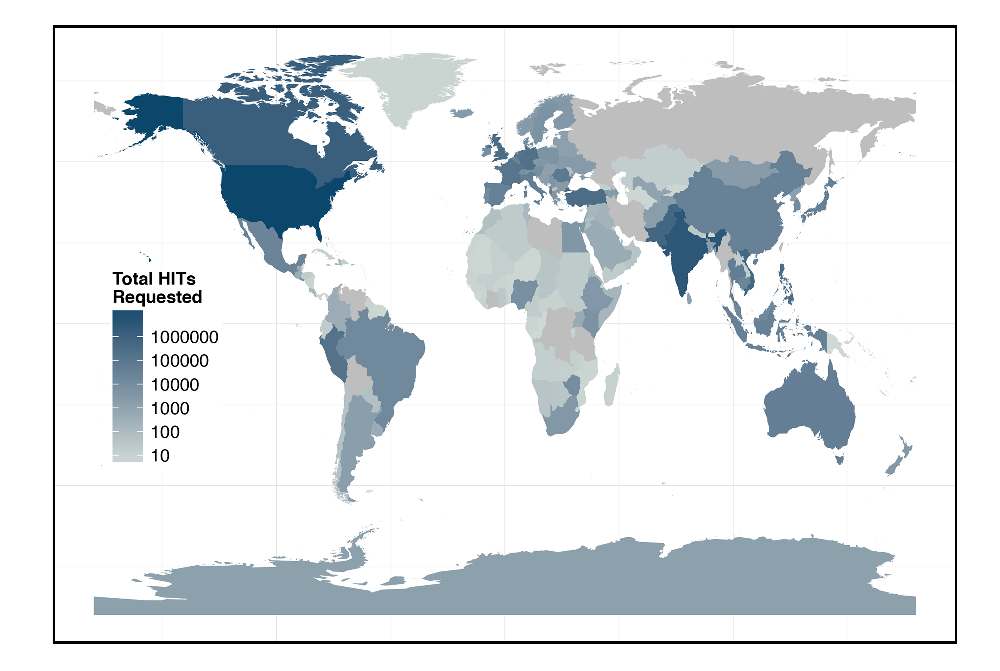
\includegraphics[width=0.43\textwidth]{figures/map}
		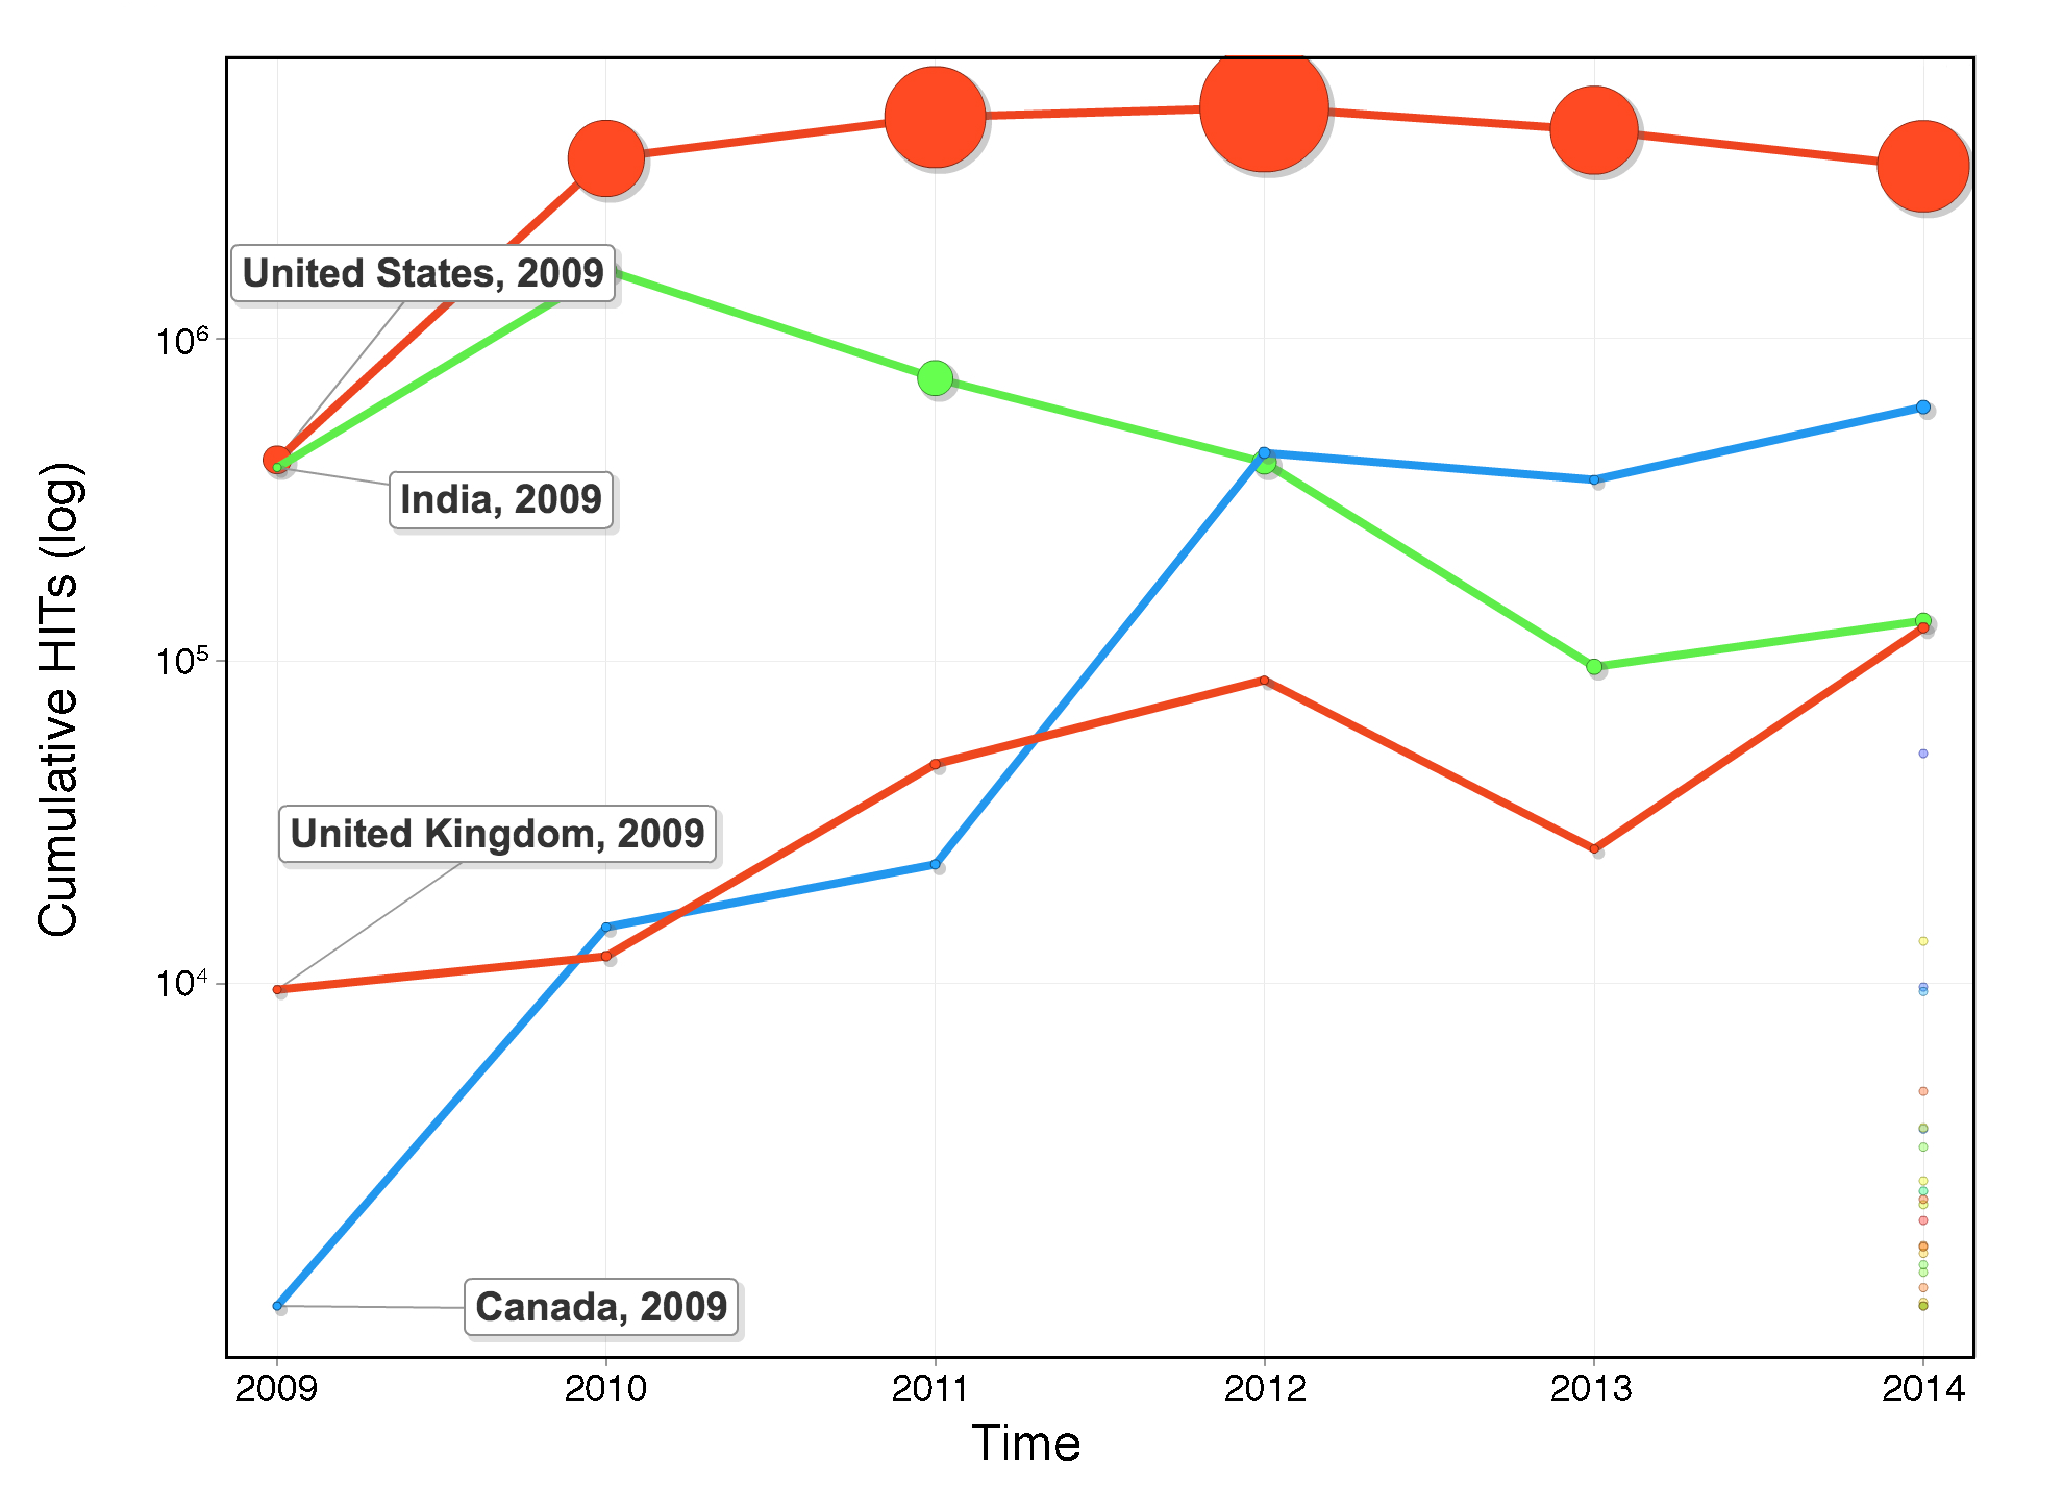
\includegraphics[width=0.43\textwidth]{figures/countriesTime}
	\caption{HITs with specific country requirements. On the left-hand side, the countries with most HITs dedicated to them. On the right-hand side, the time evolution (x-axis) of country-specific HITs with volume (y-axis) and reward (size of data point) information.}
	\label{fig:country}
\end{figure*}

\footnotetext{For readability, this graph represents a subset of 3 months.}

\paragraph{Preferred Countries by Requesters Over Time}
Figure \ref{fig:country} shows the requirements set by requesters with respect to the countries they select workers from. The left part of Figure \ref{fig:country} shows that most HITs are to be completed exclusively by workers located in the US, India, or Canada. The right part of Figure \ref{fig:country} shows the evolution over time of the country requirement phenomenon.
The plot shows the number of HITs with a certain country requirement (on the y-axis) and its time evolution (on the x-axis) with yearly steps. The size of the data point indicates the total reward associated to those HITs.

We observe that US-only HITs dominate, both in terms of their sheer number as well as in terms of the reward associated to them. 
Interestingly, we notice how HITs for workers based in India have been decreasing over time. This can be explained by \amt{} restrictions on accepting new workers on the platform.
On the other hand, HITs for workers based in Canada have been increasing over time, becoming in 2014 larger than those exclusively available to workers based in India.  We also see that the reward associated to them is less as compared to the budget for India-only HITs.
As of 2014, both HITs for workers based in Canada or UK are more numerous that those for workers based in India.
Overall, 88.5\% of the HIT batches that were posted in the considered time period did not require any specific worker location. 86\% of those which did impose a constraint requested US-based workers.


Figure \ref{fig:keyword_loc} shows the top keywords attached to HITs restricted to specific locations.
\begin{figure}[tb]
	\centering
		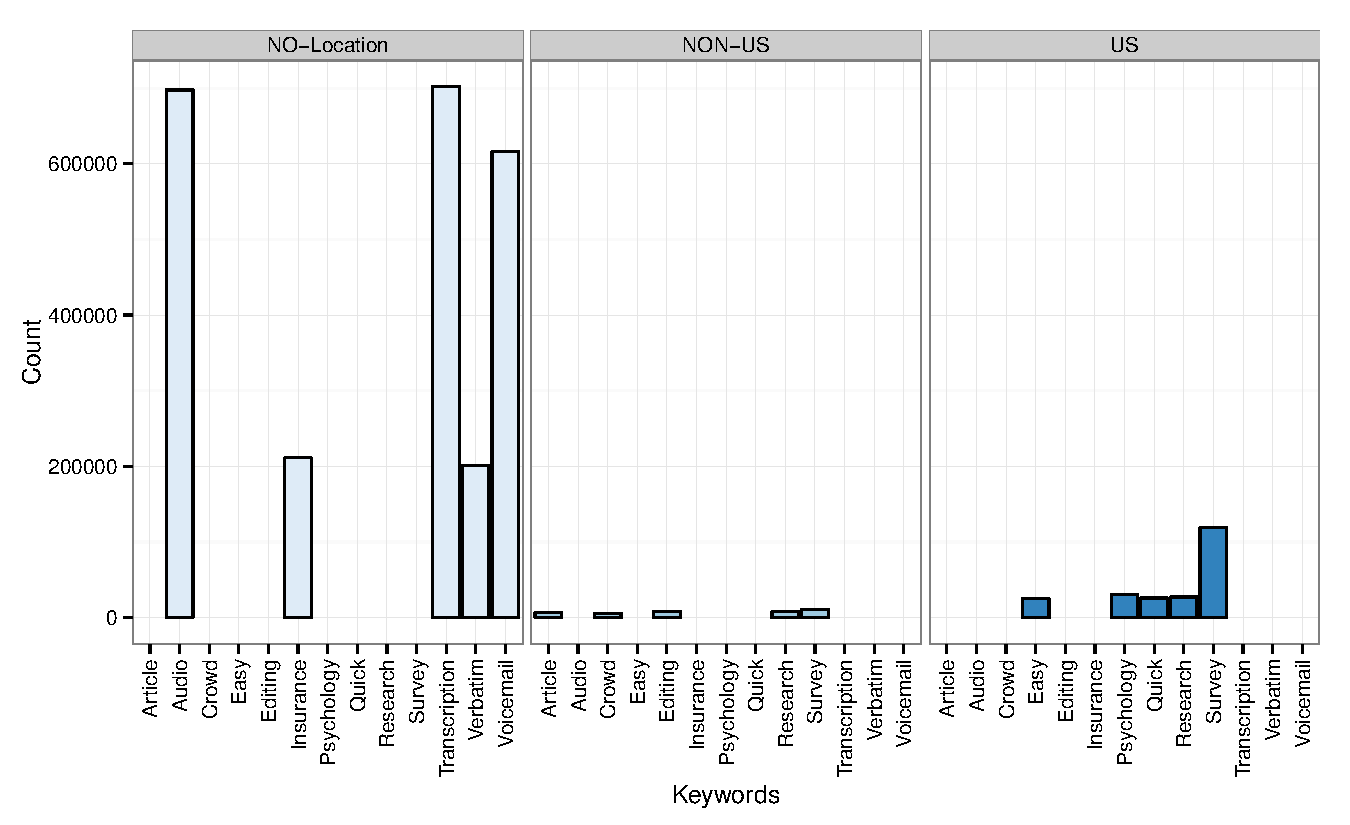
\includegraphics[width=0.5\textwidth]{figures/keywords_location}
	\caption{Keywords for HITs restricted to specific countries.}
	\label{fig:keyword_loc}
\end{figure}
We observe that the most popular keywords (i.e., `audio' and `transcription') do not require country-specific workers. This suggests that restricting workers from a single country for large batches would make their completion much slower. We also note that US-only HITs are most commonly tagged with `survey'.

% \subsection{Why Did Certain Requesters Quit?}
% \subsection{Does reputation Improve Throughput?}

\paragraph{HIT Reward Analysis}
Figure \ref{fig:reward_year} shows the most frequent rewards assigned to HITs over time\footnote{Data for 2014 has been omitted as it is not comparable with other year values.}. We observe that while in 2011 the most popular reward was \$0.01, recently HITs paid \$0.05 are getting more frequent. This can be explained both by how workers search for HITs on \amt{} and by the \amt{} fee scheme. Requesters now prefer to publish more complex HITs possibly with multiple questions in them and grant a higher reward: This also attracts those workers who are not willing to complete a HIT for small rewards and reduces the fees paid to \amt{}, which are computed based on the number of HITs published on the platform.

\begin{figure}[tb]
	\centering
		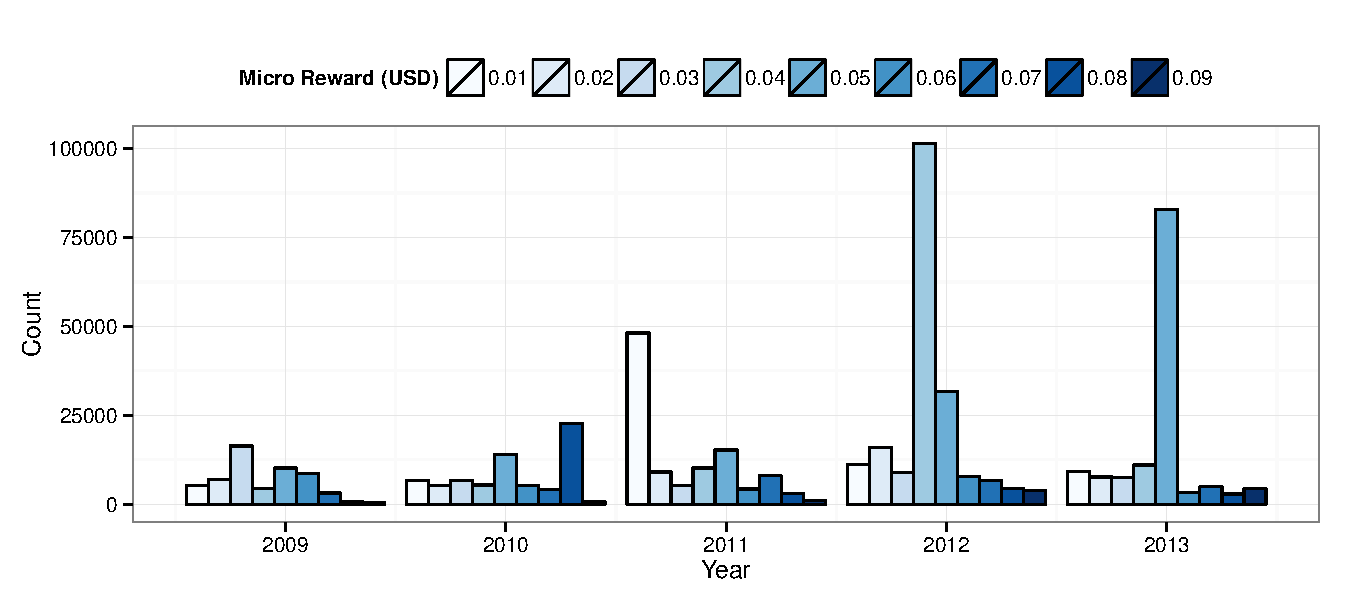
\includegraphics[width=0.5\textwidth]{figures/reward_year}
	\caption{Popularity of HIT reward values over time.}
	\label{fig:reward_year}
\end{figure}



\paragraph{Requester Analysis}
In order to be sustainable, a crowdsourcing platform needs to retain requesters over time or get new requesters to replace those who do not publish HITs anymore. Figure \ref{fig:requesters_reward} shows the number of new requesters who used \amt{} and the overall number of active requesters at a certain point in time. We can observe an increasing number of active requesters over time and a constant number of new requesters who join the platform (at a rate of 1000/month over the last two years).

\begin{figure}[tb]
	\centering
		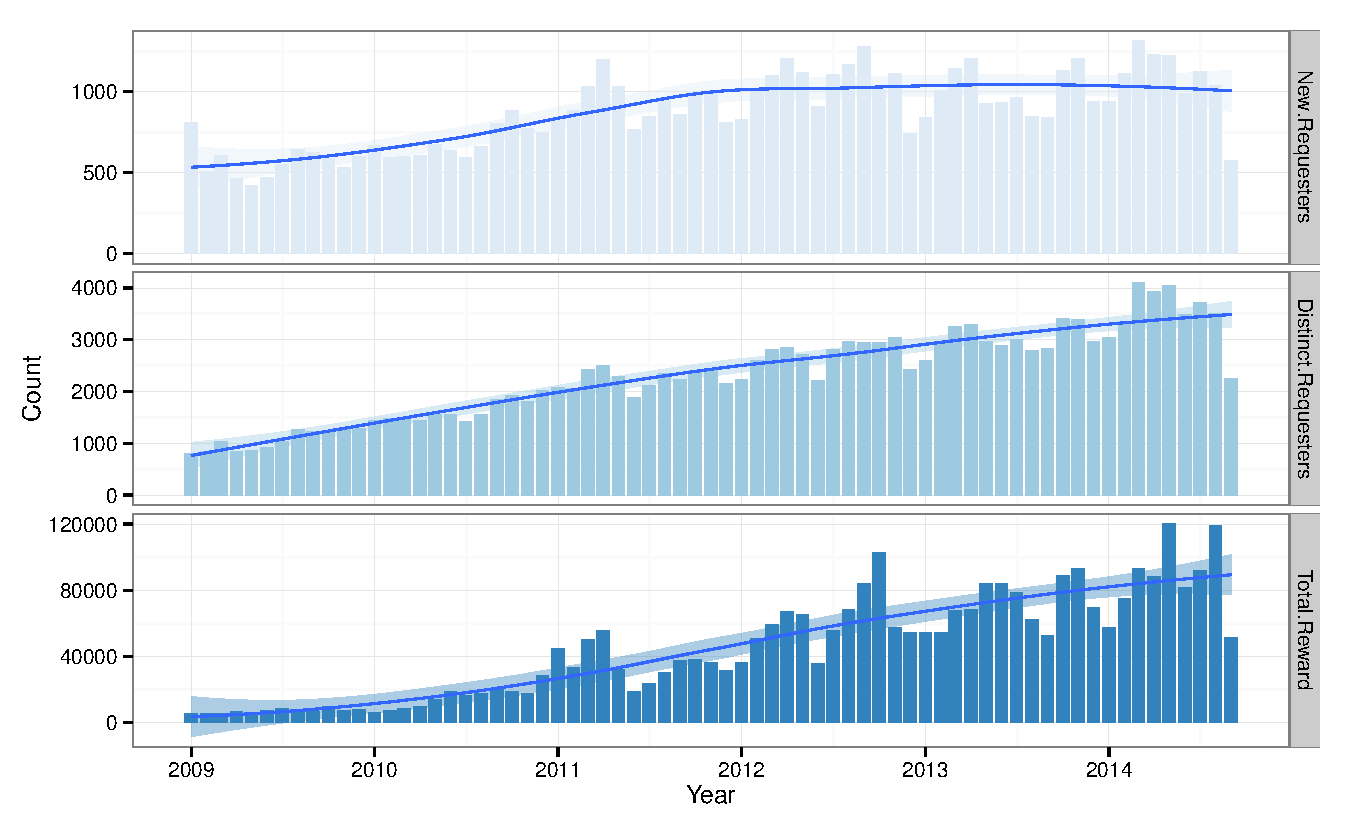
\includegraphics[width=0.5\textwidth]{figures/requesters_reward}
	\caption{Requester activity and total reward on the platform over time. The line over the data shows local polynomial regression fitting \cite{cleveland1992local}.}
	\label{fig:requesters_reward}
\end{figure}

It is also interesting to look at the overall amount of reward for HITs  published on the platform, as platform revenues are computed as a function of HIT rewards. From the bottom part of Figure \ref{fig:requesters_reward}, we  observe a linear increase in the total reward for HITs on the platform. Interestingly, we also observe some seasonality effects over the years, with October being the month with the highest total reward and January or February being the month with minimum total reward.


\paragraph{HIT Batch Size Analysis}
When a lot of data needs to be crowdsourced (like many images to tag), multiple  tasks containing similar HITs can be published together. We define a batch of HITs as a set of similar HITs published by a requester at a certain point in time. Figure \ref{fig:batch_size} shows how batch size has changed over time.
We can see that while, on average, batches have been getting smaller, in 2014 very large batches have appeared on \amt{}, indicating a clear business interest and scalability demand for micro-task crowdsourcing.

\begin{figure}[tb]
	\centering
		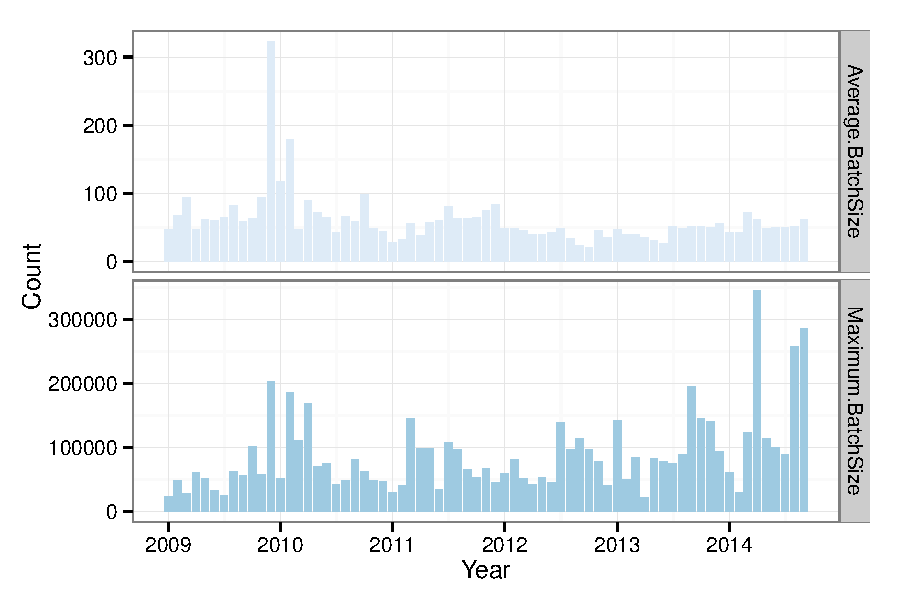
\includegraphics[width=0.5\textwidth]{figures/batch_size}
	\caption{Batch Sizes. The line over the data shows local polynomial regression fitting \cite{cleveland1992local}.}
	\label{fig:batch_size}
\end{figure}



%!TEX root = ../dynamics.tex
\section{Large-Scale HIT Type Analysis}\label{sec:type}
In this section we present the results of a large-scale analysis of the evolution of HIT \emph{types} published on the \amt{} platform.
For such analysis we use the definition of HIT types proposed by \cite{Gadiraju:2014:TMW:2631775.2631819} in which authors perform an extensive study involving 1000 crowd workers to understand their working behavior. 

\subsection{A Classification of HIT Types}
Next, we describe the six top-level classes as introduced by \cite{Gadiraju:2014:TMW:2631775.2631819}.

\begin{itemize}[noitemsep,topsep=0pt,parsep=0pt,partopsep=0pt]

	\item Information Finding (IF): Searching the Web to answer a certain information need. For example, ``Find the cheapest hotel with ocean view in Monterey Bay, CA''.
	
	\item Verification and Validation (VV): Verifying certain information or confirming the validity of a piece of content. Examples include checking Twitter accounts for spamming behaviors.

	\item Interpretation and Analysis (IA): Interpreting Web content. For example, ``Categorize product pictures in a predefined set of categories'', or ``Classify the sentiment of a tweet''.
	
	\item Content Creation (CC): Generating new content. Examples include summarizing a document  or transcribing an audio recording.

	\item Surveys (SU): Answering a set of questions related to a certain topic (e.g., demographics or customer satisfaction). 
	
	\item Content Access (CA): Accessing some Web content. Examples include watching on-line videos or clicking on provided links.

\end{itemize}

\subsection{Supervised HIT Type Classification}
Using the definition of HIT types described above, we trained a supervised machine learning model to classify HIT types based on their metadata. The features we used to train a Support Vector Machine (SVM) model are: HIT title, description, keywords, reward, date, allocated time, and batch size.

% labelling setup
To train and evaluate the supervised model we created labelled data: We uniformly sampled 5000 HITs over the entire five-years dataset and manually labelled their type by means of crowdsourcing. In detail, we asked workers on MTurk to assign each HIT to one of the predefined classes by presenting them with the title, description, keywords, reward, date, allocated time, batch size for the HIT. The instructions also contained the definition and examples for each task type. Workers could label tasks as `Others' when unsure or when the HIT did not fit in any of the available options.

% labelled data
After assigning each labelling HIT to three different workers in the crowd, a consensus on the task type label was reached in $89\%$ of the cases (i.e., 551 cases with no clear majority). A consensus was reached when at least two out of three workers agreed on a HIT type label. The other cases, that is, when the workers provided different labels or when they where not sure about the HIT type have been removed from our labelled dataset.

% classification evaluation
Using the labelled dataset we trained a multi-class SVM classifier for the 6 different task types and evaluated its quality with 10-folds cross validation over the labelled dataset. Overall, the trained classifier obtained Precision of $0.895$, Recall of $0.899$, and F-Measure of $0.895$. Most of the classifier errors (i.e., 66 cases) were done by incorrectly classifying IA instances as CC.

% top features
Performing feature selection for the HIT type classification problem we observed that the best features according to information gain are the HIT allotted time and reward: This indicates that HITs of different types are associated with different levels of reward as well as different task duration (i.e., longer and better paid tasks versus shorter and paid worse). 
Most distinctive keywords for identifying HIT type are `transcribe', `audio', and `survey' which clearly identify CC and SU HITs.
 
% classification at scale
Using the classifier trained over the entire labelled dataset, we then performed a large scale classification of the type for all 2.5M HITs in our collection. This allows us to study the evolution over time of task types on the \amt{} platform which we present next.

\subsection{Task Type Popularity Over Time}
Using the result of the large-scale classification of HIT types, we  analyze which  types of HITs have been published over time.
Figure \ref{fig:cat_trends} shows the evolution of task types published on \amt{}\ .
% 
We can observe that, in general, the most popular type of task is Content Creation.
% 
In terms of observable trends, we note that, while there is a general increase of the volume of tasks of a certain type on the platform,  CA tasks have been decreasing over time. This can be explained  by the enforcement of \amt{} terms of service which state that workers should not be asked to create accounts on external website or be identified by the requester.
% 
In the last three years, SU and IA tasks have had the biggest increase.

\begin{figure}[htbp]
	\centering
		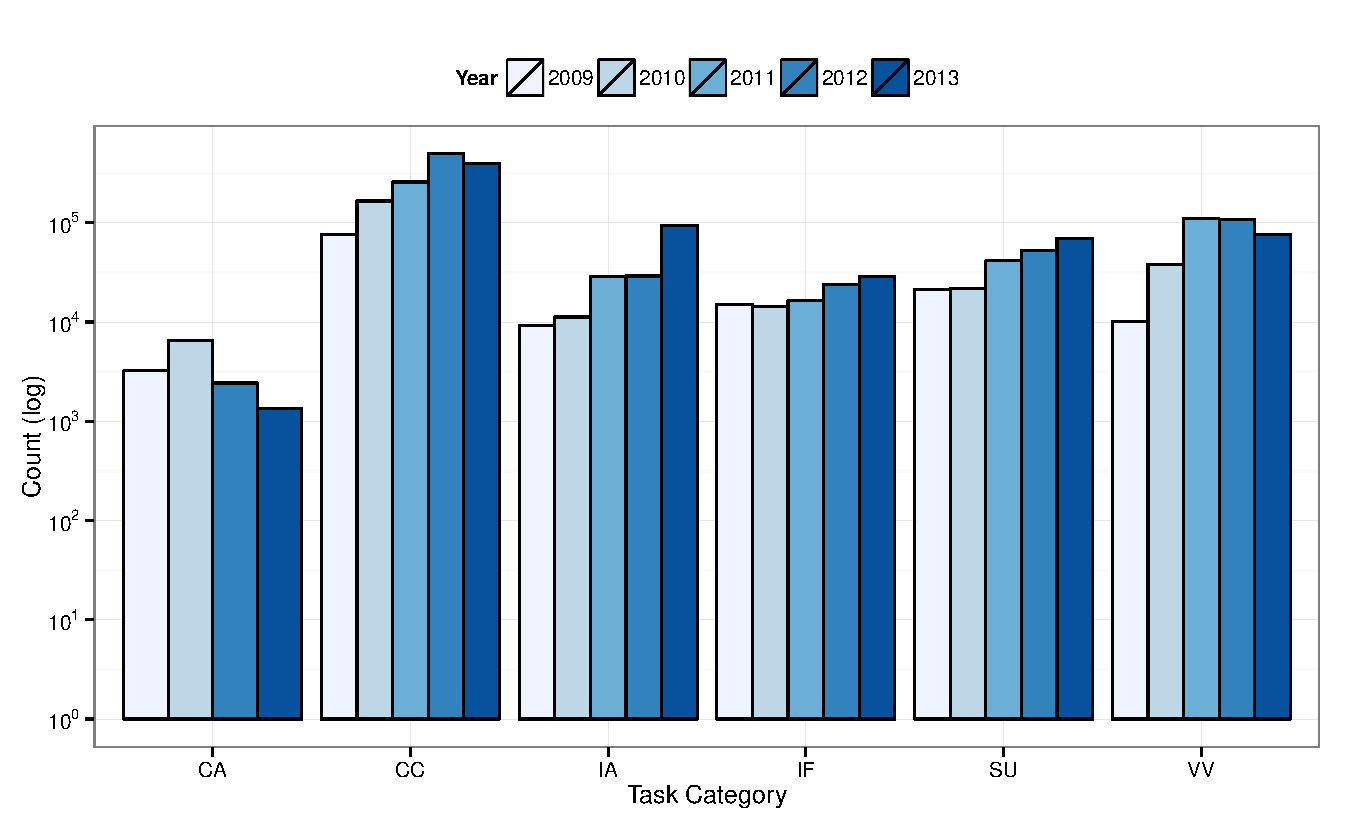
\includegraphics[width=0.5\textwidth]{figures/category_trends}
	\caption{Popularity of HIT types over time.}
	\label{fig:cat_trends}
\end{figure}


%!TEX root = ../dynamics.tex
\section{Analyzing the Features Affecting Batch Throughput}
\label{sec:throughput}
Next, we turn our attention to analyzing the factors that influence the progress (or the pace) of a batch, how those factors influence each other and how their importance changes over time. 

In order to conduct this analysis, we try to predict the throughput of a batch of tasks (or how many HITs get will get completed in the next time frame). 
The value we aim to predict is the batch \emph{throughput}, that is, the numbers of HITs that  will be completed for a given batch within the next time frame of 1 hour (i.e.,  the $DIFF\_HIT$ feature is a target class).
Specifically, we model this task as a regression problem using 29 features; some of them were used in the previous section to classify HIT type, we describe the remaining ones in Appendix A.

\subsection{Experimental Setup}

To predict the throughput of a batch at time $T$, we train a Random Forest Regression model with samples taken in the range $[T-\delta, T)$ where $\delta$ is the size of the time window that we are   considering directly prior to time $T$. The rational behind this approach is that the throughput should be directly correlated to the current and recent market situations. 
The research question we tackle in this context is:\\ \emph{``How much historical data does one need to consider to predict the throughput effectively?"}. \\ To answer this, we proceed by varying $\delta$.
To evaluate the effectiveness of $\delta$ values, we compute the coefficient of determination  $R^2$ \cite{sklearnweb, sklearn}.
In this experiment, we considered  data from June to October 2014 and hourly observations (see Section \ref{sec:tracker}), from which we uniformly sampled 50 time points for evaluation purposes. Finally, for each time point we considered a training time frame $\delta$ ranging from 1 hour to 24 hours. 

\subsection{Prediction}
In Figure \ref{fig:accuracy}, we observe that the computed evaluation score reaches its highest values when using the latest 4 hours as training time-frame, then decreases when we increase the training time-frame, to finally again increase and stabilize when we use up to 24 hours training data.
Note that the score is relatively low for batches with low throughput. 

Our prediction results (when using 4hours window) versus actual throughput values are shown in Figure \ref{fig:pred}. The prediction works best for larger batches having a large momentum as the Figure suggests.

\begin{figure}[t!]
	\centering
		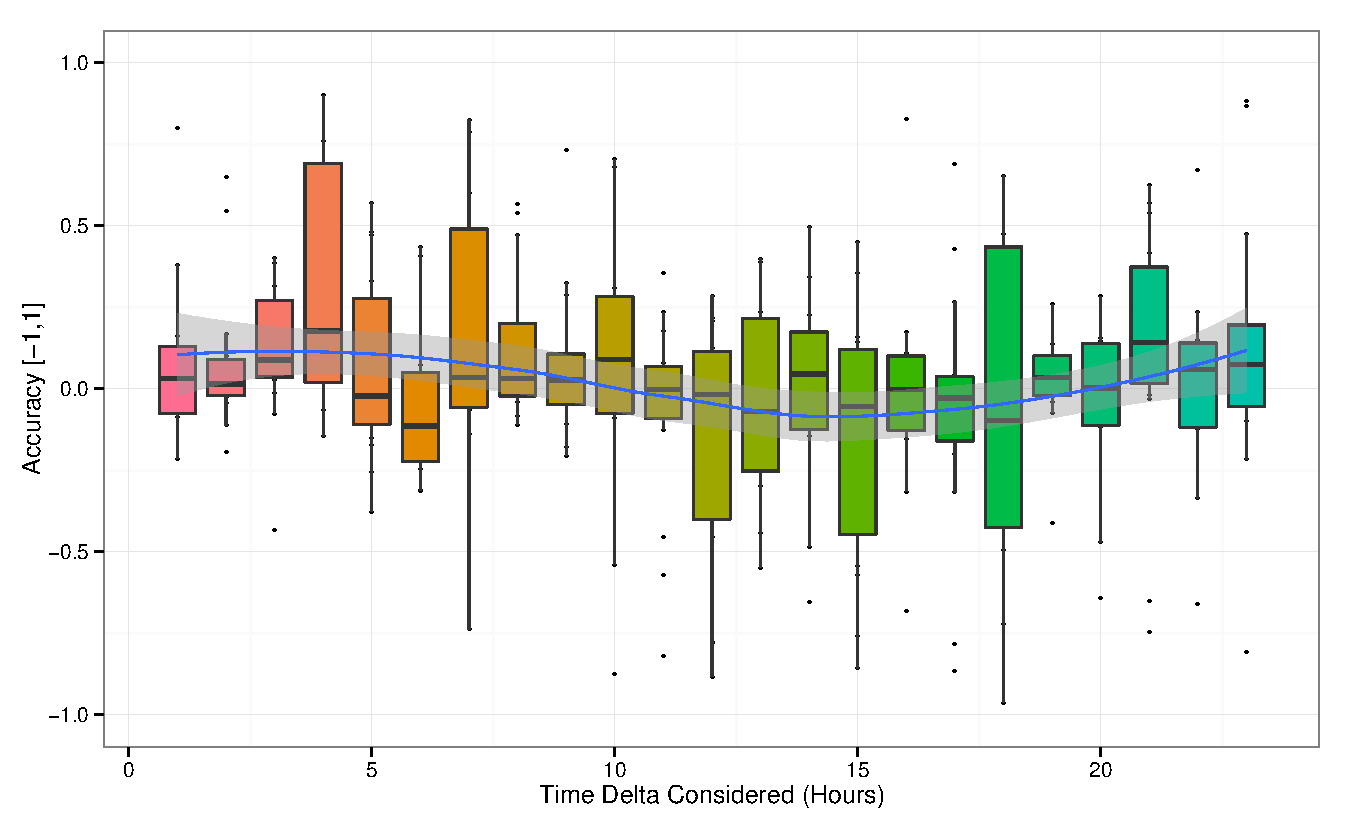
\includegraphics[width=0.48\textwidth]{figures/ML_accuracy}
	\caption{Score ($R^2$) of the throughput prediction when considering larger time spans as training sets. The red dots are average values, while the boxes represents the median, first and third quartiles. N.B., the implementation of the score function used in our experiments allows for negative values.}
	\label{fig:accuracy}
\end{figure}
\footnotetext{\url{http://scikit-learn.org/stable/modules/generated/sklearn.metrics.r2_score.html}}

\begin{figure}[t!]
	\centering
		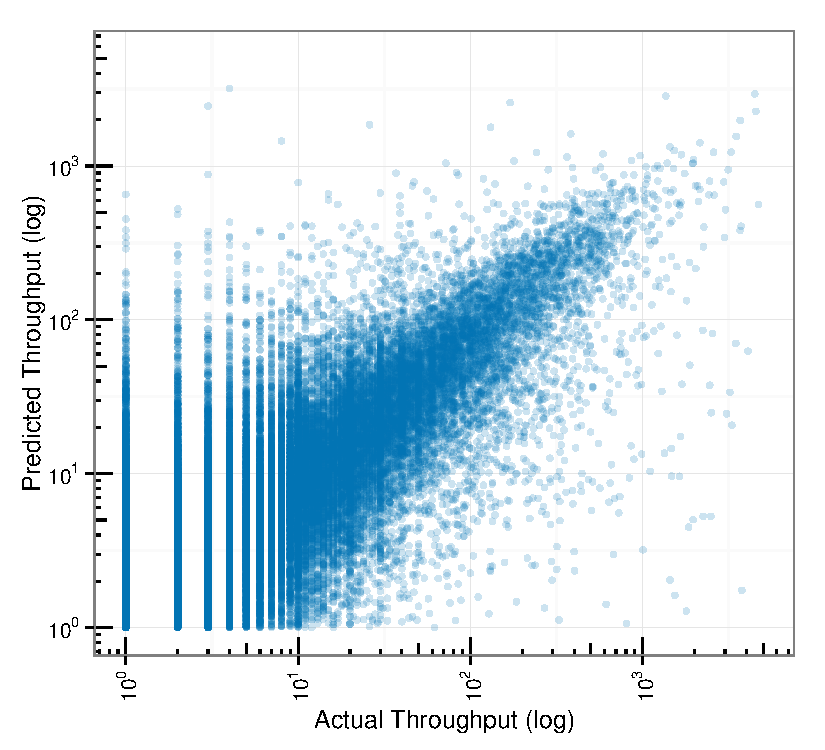
\includegraphics[width=0.48\textwidth]{figures/predictions_3}
	\caption{Prediction vs actual throughput values. Prediction is more accurate for larger throughput values. This suggests that the throughput will remain high until the batch gets smaller.}
	\label{fig:pred}
\end{figure}

\subsection{Features Importances}
In order to better grasp the characteristics of the batch throughput, we examine the prediction's features importances to understand which ones contributes more.

Figure \ref{fig:importances} shows the  contribution of the top 4 features and how it varies  when we increase the training time-frame. The rest of the features importances are listed in Table \ref{table:feats}, their slope indicates whether the feature is gaining importance overtime (positive value) or decreasing in importance (negative value).
The most important feature is $HIT\_Available$, that is, the current size of the batch. Indeed, as observed by previous work, larger batches tend to attract more workers \cite{mturk,crowddb}. This feature becomes less important when we consider longer periods, partly because of noise, but, most importantly, because of other features like $age\_minutes$ and $left\_minutes$, which encode additional facts and suggest that the crowd is sensitive to the newly posted HITs, or how \emph{fresh} the HITs are. To better understand this phenomenon, we conduct an analysis on what attracts the workforce to the the platform in the next section.

\begin{figure}[t!]
	\centering
		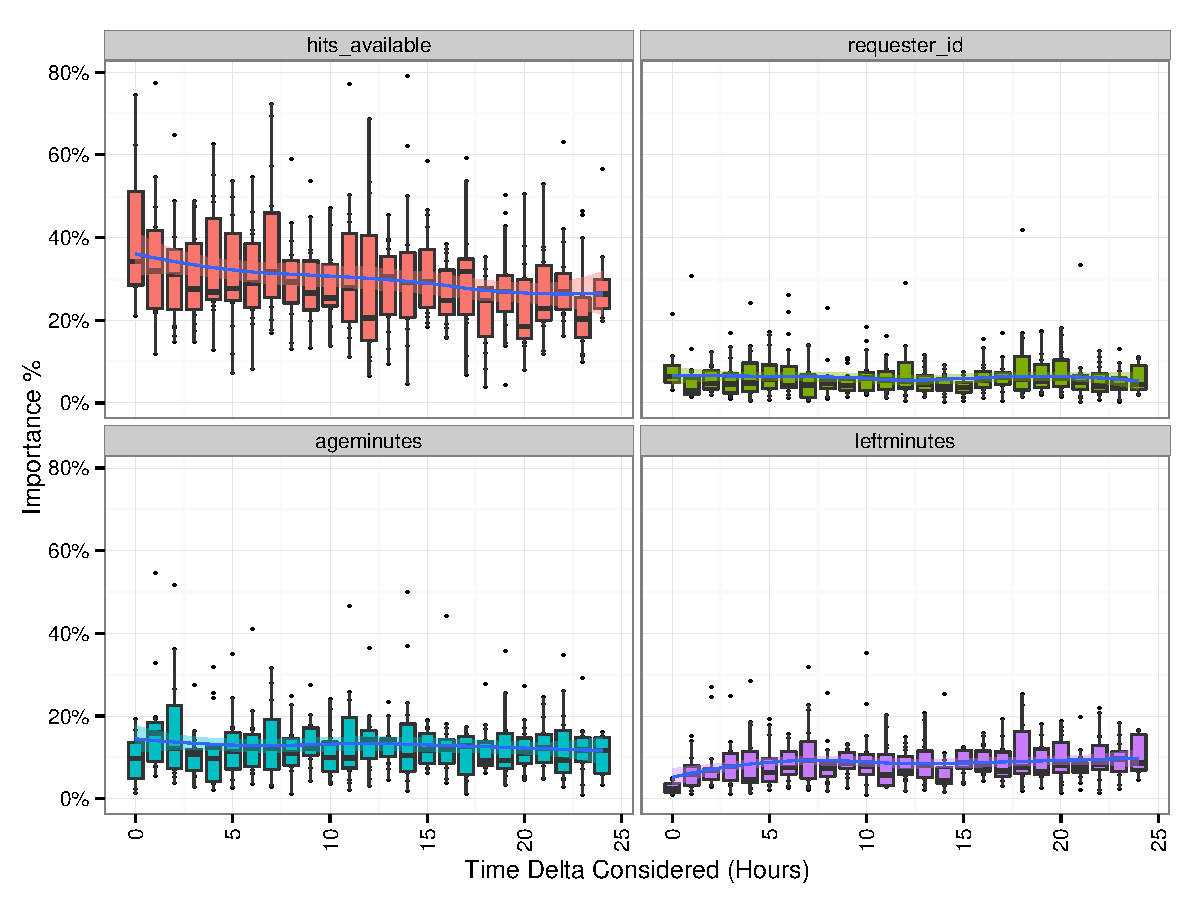
\includegraphics[width=0.5\textwidth]{figures/importances}
	\caption{Computed feature importance when considering larger training sets for the prediction.}
	\label{fig:importances}
\end{figure}


\begin{table}[t!]
\scriptsize
\begin{tabular}{|c|c|c|c|c|}
\hline
Feature              & mean      & stddev    & slope     & intercept \\
\hline
hits\_available      & 29.8606 & 13.4247 & -0.0257 & 34.4940 \\
ageminutes           & 12.9087 &  8.1967 & -0.0050 & 13.8181 \\
leftminutes          &  8.7300 &  5.5530 & 0.0061 & 7.6290 \\
requester\_id        &  6.2147 &  5.2943 & -0.0011 & 6.4305 \\
title                &  5.6441 &  4.2604 & -0.0033 & 6.2519 \\
description          &  4.8823 &  3.8975 & -0.0065 & 6.0617 \\
keywords             &  4.3765 &  3.3860 & -0.0074 & 5.7095 \\
time\_alloted        &  3.7994 &  3.6820 & -0.0010 & 3.9965 \\
reward               &  3.5439 &  2.7426 & -0.0011 & 3.7458 \\
totalapproved        &  2.5259 &  3.5108 & 0.0033 & 1.9311 \\
tasktype             &  2.1370 &  2.2673 & -0.0008 & 2.2986 \\
start\_time          &  1.2257 &  1.4123 & 0.0049 & 0.3325 \\
hitsAvailableUI      &  1.1428 &  1.2062 & 0.0039 & 0.4380 \\
diffHitsUI           &  1.0557 &  1.1237 & 0.0038 & 0.3568 \\
hitGroupsAvailableUI &  1.0438 &  1.0219 & 0.0034 & 0.4169 \\
diffGroupsUI         &  1.0408 &  1.0658 & 0.0030 & 0.4835 \\
master               &  0.9943 &  2.3816 & -0.0012 & 1.2134 \\
diffGroups           &  0.9660 &  0.9349 & 0.0032 & 0.3863 \\
rewardsArrived       &  0.9543 &  1.0710 & 0.0032 & 0.3698 \\
hitsCompleted        &  0.9293 &  0.9453 & 0.0031 & 0.3593 \\
percHitsCompleted    &  0.8974 &  0.8548 & 0.0030 & 0.3543 \\
location             &  0.8957 &  1.7592 & 0.0004 & 0.8184 \\
diffRewards          &  0.8920 &  0.8967 & 0.0023 & 0.4622 \\
rewardsCompleted     &  0.8890 &  0.8896 & 0.0026 & 0.4056 \\
percHitsPosted       &  0.8462 &  0.9552 & 0.0021 & 0.4618 \\
diffHits             &  0.8462 &  0.7514 & 0.0024 & 0.3972 \\
hitsArrived          &  0.7562 &  0.7946 & 0.0021 & 0.3760 \\
approvalrate         &  0.0000 &  0.0000 & 0 & 0 \\
\hline
\end{tabular}
\caption {Importances of the features used in the prediction experiment. A large mean indicates a better overall contribution to the prediction. A positive slope indicates that the feature is gaining in importance when the considered time window increases.}
\label{table:feats}
\end{table}
%!TEX root = ../dynamics.tex
\section{Market Analysis}
\label{sec:market}
Finally, we study the demand and supply of the Amazon MTurk marketplace. In the following, we define $Demand$ as the number of new tasks published on the platform by the requesters. In addition, we compute the average reward of the tasks that were posted. Conversely, we define $Supply$ as the workforce that the crowd is providing, concretized as the number of tasks that got completed in a given time window by the workers. %Again, we compute the average reward of the completed tasks.
In this section we use hourly collected data for the time period spanning June to October 2014.

%\subsection{Supply vs. Demand}
%First, we check whether supply and demand, in the context of Amazon MTurk marketplace, exhibit the standard behavior and relationship.
%Figure \ref{fig:dsup} (right) shows the expected relationship between supply and price: The larger the supply, the lower the price evolves, which is the usual behavior in a market. On the other hand, Figure \ref{fig:dsup} (left) shows that the demand does not match the typical ascending demand curve (``the higher the demand the higher the price evolves''). Instead, the demand seems to be tied to the supply (i.e., the number of new HITs completed).
%
%\begin{figure}[t!]
%	\centering
%		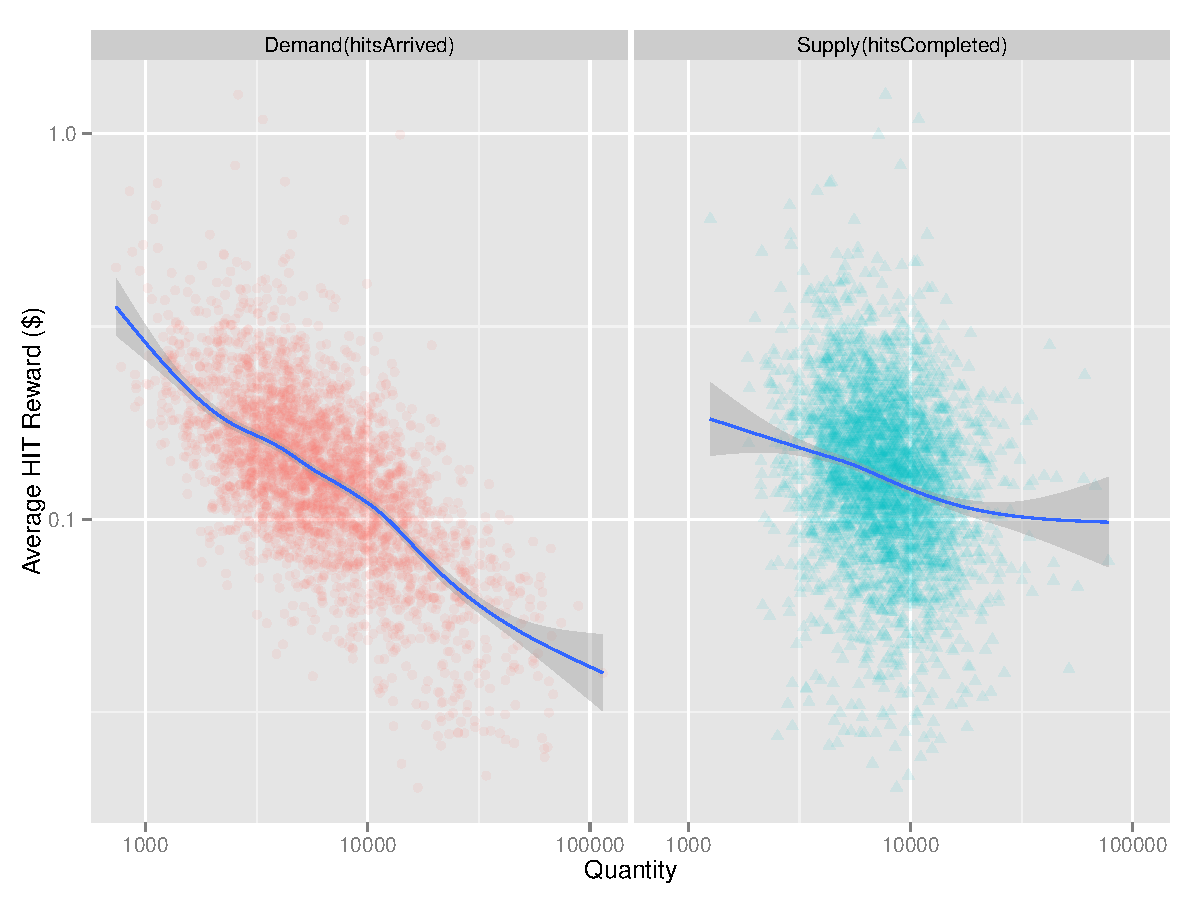
\includegraphics[width=0.48\textwidth]{figures/ds}
%	\caption{The supply and demand for HITs versus the average HIT price.}
%	\label{fig:dsup}
%\end{figure}

\subsection{Supply Attracts New Workers} %

%Now, we examine how the supply attracts new workers. First, we compare the three following variables: number of HITs published on the platform, number of HITs completed, and the average reward per HIT of both published and completed tasks. The results are depicted in Figure \ref{fig:scatter_matrix}. The apparent correlation between the rewards of the HITs completed and those published, and also among their quantities, gives us a first intuition that the crowd workers are sensitive to newly posted tasks, especially for those with higher prices.
%
%\begin{figure}[t!]
%	\centering
%		
\includegraphics[width=0.48\textwidth]{figures/scatter}
%	\caption{Scatter matrix comparing the different parameters in the demand and supply.}
%	\label{fig:scatter_matrix}
%\end{figure}

We start by analyzing how the market reacts when new tasks arrive on the
platform, in order to understand the degree of elasticity of the supply. If the supply of work is inelastic, the amount of work done over time should
be independent of the demand for work. So, if the amount of tasks
available in the market (``demand'') increases, then the percentage of
work that gets completed in the market should drop, as the same amount of ``work done" gets split among a higher number of tasks. To
understand the elasticity of the supply, we regressed the percentage of
work done in every time period (measured as the percentage of HITs
that are completed) against the number of new HITs that are posted in
that period. Figure \ref{fig:perc_hits_completed} shows the scatterplot for those two variables.

Our data reveals that an increase in the number of arrived HITs is
positively associated with a higher percentage of completed HITs. This
result provides evidence that the new work that is posted is more
attractive than the tasks previously available in the market, and attracts ``new
work supply".\footnote{From the data available, it is not possible to tell
whether the new supply comes from distinct
workers, from workers that were idle, or from an increased productivity
of existing workers.}

Our regression\footnote{We use Ordinary Least Squares regression.} of the ``Percent Completed" against ``Hits Arrived (in
1000's)" indicates an intercept of 2.5 and a slope of 0.05. To put
these numbers in context: On average, there are 300K
HITs available in the market at any given time, and on average 10K new HITs arrive
every hour. The intercept of 2.5 means that 2.5\% of these 300K HITs
(i.e., 7.5K per hour) get completed, as a baseline, assuming that no
new HIT gets posted. The slope is 0.05, meaning that if 10K new HITs
arrive within an hour, then the completion ratio increases by
0.5\%, to 3\% (i.e., 9K HITs per hour). When 50K new HITs arrive within
an hour, then the completion percentage increases to 5\% indicating
that 15K to 20K HITs get completed. In other words, approximately 20\%
of the \emph{new} demand gets completed within an hour of being posted,
indicating that new work has almost 10x higher attractiveness for the
workers than the remaining work that is available on the platform.
% 
This result could be explained by how tasks are presented to workers by \amt{}.
Workers, when not searching for tasks using specific keywords, are presented with the most recently published tasks first.

\begin{figure}[t!]
	\centering
	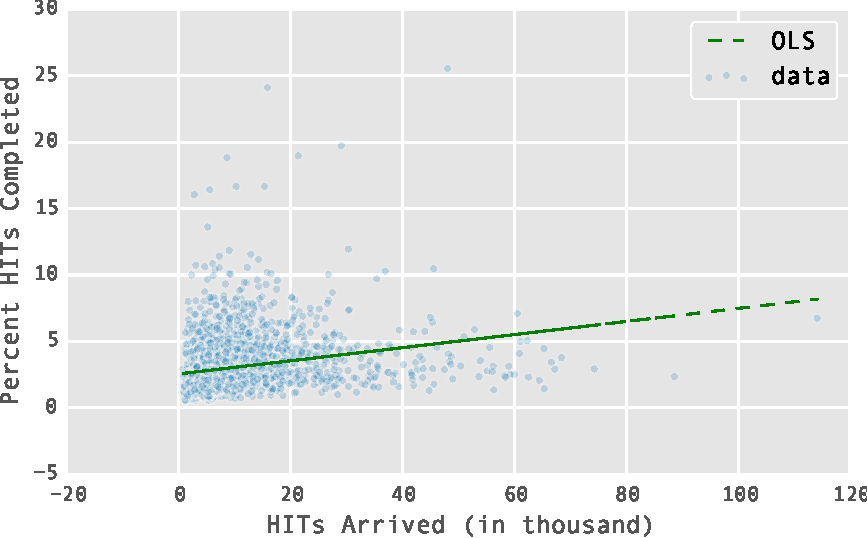
\includegraphics[width=0.48\textwidth]{figures/percent.pdf}
	\caption{The effect of new arrived HITs on the work supplied. Here, the supply is expressed as the percentage of HITs completed in the market.}
	\label{fig:perc_hits_completed}
\end{figure}

\subsection{Demand and Supply Periodicity}
On the demand side, some requesters frequently post new batches of recurrent tasks. Hence, we are interested in the periodicity of such demand in the marketplace and the supply it drives. To look in this, we consider both the time-series of available HITs and the rewards completed. 

First, we observe that the demand exhibits a strong weekly periodicity, which is reflected by the autocorrelation that we compute from the number of available HITs on Amazon Mturk (See Figure \ref{fig:hitav} and \ref{fig:achitav}). The market seems to have a significant memory that lasts for approximately 7-10 days.
This indicates that future transactions are highly predictable using simple algorithms \cite{marketmemory}.

Conversely, and to check for the periodicity in the supply, we compute an autocorrelation on the weekly moving average of the completed HITs reward. Figure \ref{fig:mac} and \ref{fig:acmac} show that there is a strong weekly periodicity effect, as we observe high values in the range 0-250 hours.

\begin{figure*}[t!]
    \centering
    \begin{subfigure}[b]{0.48\textwidth}
        \centering
        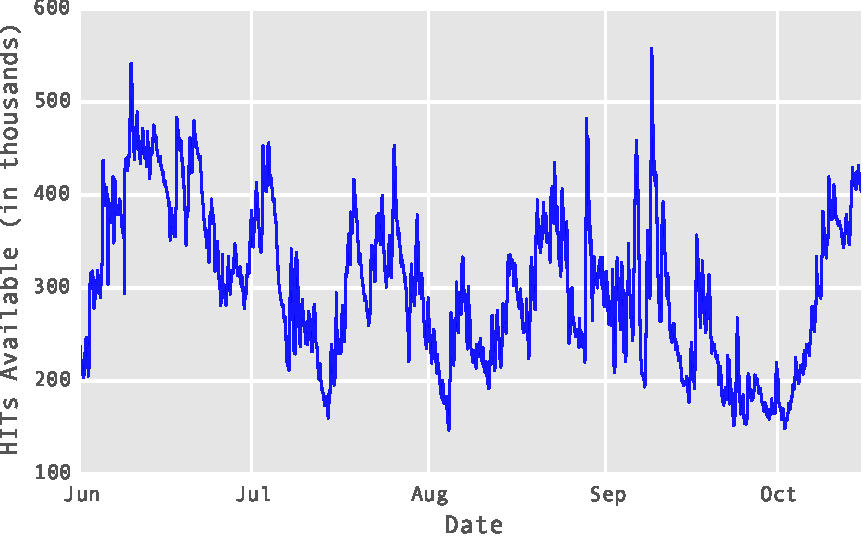
\includegraphics[width=\textwidth]{figures/out}
        \caption{HITs Available.}
        \label{fig:hitav}
    \end{subfigure}
    \hfill
    \begin{subfigure}[b]{0.48\textwidth}
        \centering
        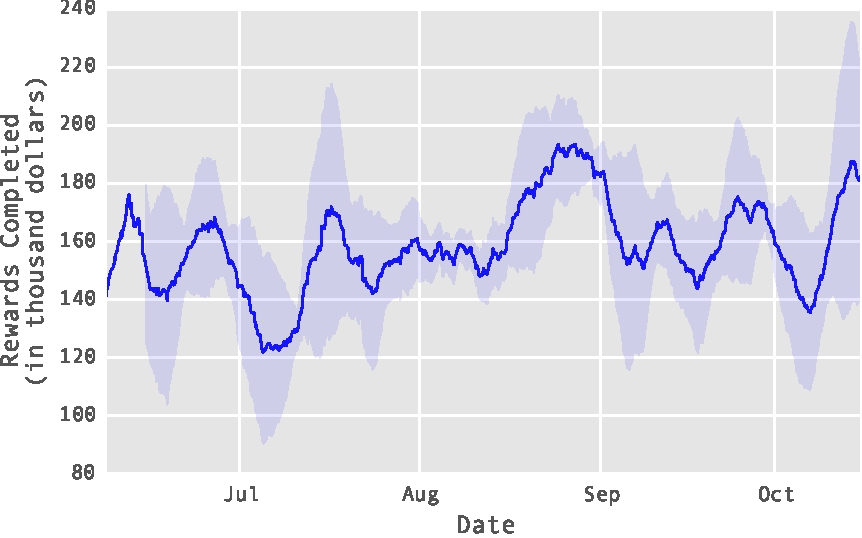
\includegraphics[width=\textwidth]{figures/mac}
        \caption{Weekly moving average on rewards completed.}
        \label{fig:mac}
    \end{subfigure}
    \hfill
    \begin{subfigure}[b]{0.48\textwidth}
        \centering
        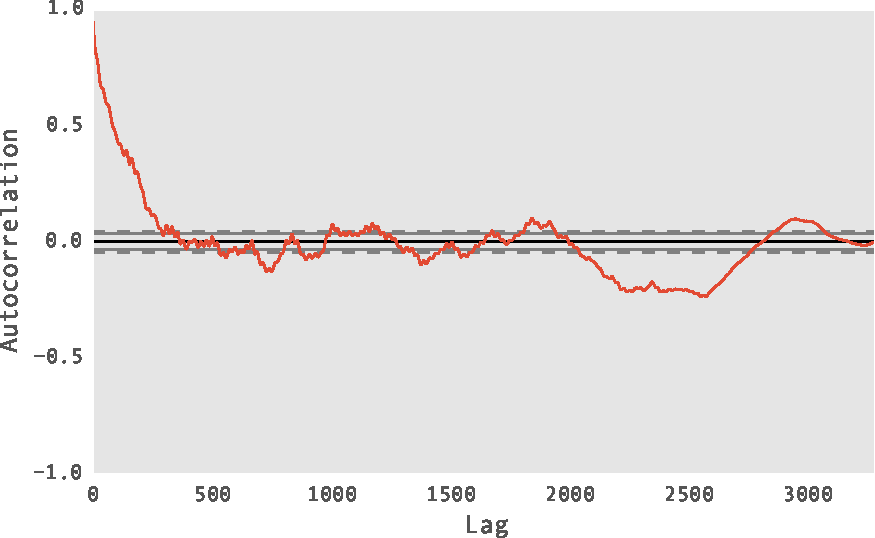
\includegraphics[width=\textwidth]{figures/out1}
        \caption{Autocorrelation on HITs available.}
        \label{fig:achitav}
    \end{subfigure}
    \hfill
    \begin{subfigure}[b]{0.48\textwidth}
        \centering
        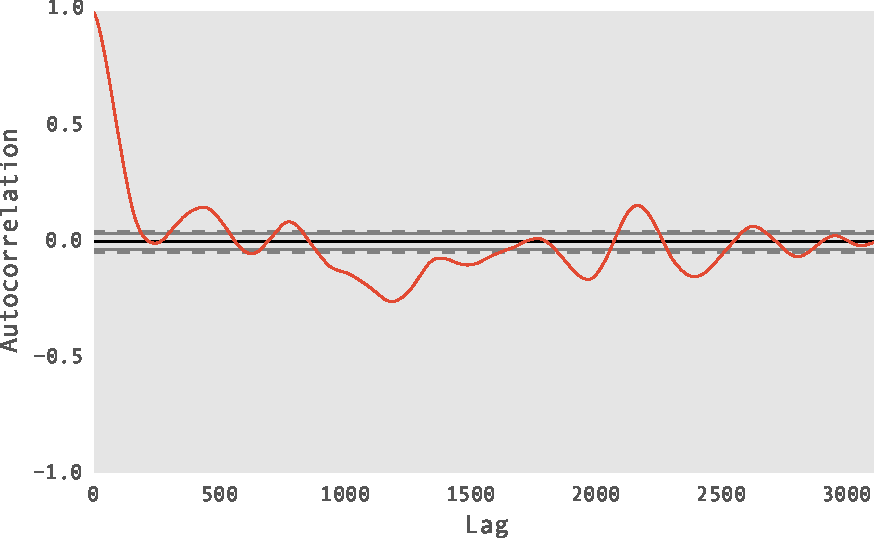
\includegraphics[width=\textwidth]{figures/macac}
        \caption{Autocorrelation on moving average of rewards completed.}
        \label{fig:acmac}
    \end{subfigure}
       
	\caption{Computed autocorrelation on the number of HITs available and on the weekly moving average of the completed reward (N.B., autocorrelation's Lag is computed in Hours). In both cases, we clearly see a weekly periodicity (0-250 Hours).}
	\label{fig:autocorrelation2}
\end{figure*}



%!TEX root = ../dynamics.tex
\section{Conclusions}\label{sec:conc}

In this paper, we presented an analysis of the evolution of micro-task crowdsourcing over the past five years.
We studied data collected from a popular micro-task crowdsourcing platform: \amt{}.
We analyzed a number of key dimensions of the platform, including: topic, task type, or reward evolution, platform throughput, supply and demand curves.
The main findings of our analysis are as follows:
\begin{itemize}[noitemsep,topsep=0pt,parsep=0pt,partopsep=0pt]
	\item Tasks related to audio transcription have been gaining momentum in the last years and are today the most popular tasks on \amt{}.
	\item The popularity of Content Access HITs has decreased over time. Surveys are however becoming more popular over time.
	\item While most HITs do not require country-specific workers, most of such HITs require US-based workers.
	\item HITs that are exclusively asking for workers based in India have strongly decreased over time.
	\item Surveys are the most popular type of HITs for US-based workers.
	\item The most frequent HIT reward value has increased over time, and reaches \$0.05 in 2014.
	\item New requesters constantly join \amt{}, making the total number of active requesters and the available reward increase over time.
	\item The average HIT batch size is constant over time; however, very large batches have recently started to appear on the platform.
	\item The throughput of HIT batches can best be predicted based on the number of HITs available in the batch (i.e., its size) and its freshness.
	\item New HITs attract new workers to the platform.
	\item New workers arriving to the platform complete both fresh and old HITs.
\end{itemize}

The results of our analysis can serve as a starting point for improving existing crowdsourcing platforms and to optimized the overall efficiency and effectiveness of human computation systems. The evidence presented above  indicate how requesters should use crowdsourcing platforms to obtain the best out of them: Engage with workers and publish large volumes of HITs at specific points in time. 

%For this purpose we created a system that can support requesters in publishing their HITs optimizing for throughput\footnote{\url{http://xi-lab.github.io/mturk-mrkt/}}.

\bibliographystyle{abbrv}
\bibliography{crowd}

\end{document}
